For the next two chapters, we will depart a little from the previous focus which was by and large on \emph{algorithms}, and look into their usual companion: \emph{data structures}. This is not saying there will not be algorithms, or analysis of algorithms, or extensive use of these concentration inequalities and mathematical notions we introduced and went over at great length! 

First, just so that we are clear on \emph{what} a data structure is: it is a way to store and organize data while providing a set of methods to access (and, usually,  update) this data \emph{efficiently}. This set of methods is the interface to the data (the analogue of an API), and you may have seen it referred in previous courses by what is called an \emph{abstract data type} (ADT). So an ADT specifies an ``API to the data,'' and a data structure is a concrete implementation of this API.\footnote{Not an implementation in terms of code, but in terms of algorithms, etc. Once you have a data structure defined and you've analyzed it, it still remains to code it at some point\dots}

Second, we will typically care about time efficiency, but also space (memory) efficiency of a data structure: if we currently store 5 $\green{m}$-bit strings, we would rather avoid using $\Theta(2^{\green{m}})$ bits of memory~--~even though in this case that's the size of the ``universe'' the data comes from (there are $2^{\green{m}}$ distinct $\green{m}$-bit strings). To quantify this, let's introduce some notation: we will have $\ns$ \emph{elements} (data points), each of them coming from a \emph{universe} (set of all possible data points) $\cX$ of size $\green{m}$. Our two main parameters will be $\ns$ and $\green{m}$: $\ns$ can increase or decrease as we add or remove elements from our data structure, and we usually have $\ns \ll \green{m}$ (the universe is big, our dataset is much smaller).

As an example: we want to store 10,000 high-resolution pictures, each 12.5 MP ($3072 \times 4080$ resolution). Assuming 8 bits per pixel, what would be the corresponding values of $\ns$ and $\green{m}$?\marginnote{This is a very naive way to bound $\green{m}$, as not all sets of pixels will be valid images. But it is good enough as a first approximation.}
\begin{itemize}
    \item $\ns=10,000$ and $\green{m} = 12,533,760$?
    \item $\ns=10,000$ and $\green{m} = 100,270,080$?
    \item $\ns=10,000$ and $\green{m} = 2^{100,270,080}$?
\end{itemize}
Clearly, we do not want to use space proportional to $\green{m}$.\medskip

Now, one of the most basic and fundamental examples of ADTs is that of the \emph{dictionary},\marginnote{Or \emph{map}, or \emph{associative array.}} which only requires to provide 3 operations to maintain a set $S\subseteq \cX$:
\begin{framed}
    \begin{itemize}
        \item$\textsc{Insert}(x)$: insert the element $x$ to $S$ (do nothing if it is already in $S$)
        \item$\textsc{Lookup}(x)$: return whether $x\in S$
        \item$\textsc{Remove}(x)$: remove the element $x$ from $S$ (do nothing if it is not in $S$)
    \end{itemize}
\end{framed}
Of course, there are several options to implement this, and you most likely have seen or easily come up with a few data structures for that:\marginnote{Check how you would get these. Can you think of others?}
\begin{itemize}
    \item A linked list! Space $O(\ns \log \green{m})$, all three operations in (worst-case) time $O(\ns)$.
    \item An array! Space $O(\green{m})$, all three operations in (worst-case) time $O(1)$.
    \item A self-balancing binary search tree (BST), \eg an AVL tree! Space $O(\ns \log \green{m})$, all three operations in (worst-case) time $O(\log\ns)$.
\end{itemize}
Each of these has its drawbacks, especially the first two. Is there a way to do better? Specifically, can we do space $O(\ns)$ \emph{and} all three operations in time complexity $O(1)$?\medskip

\noindent Not quite, but \emph{almost}. Enter {hash tables}, which, at a high level, use randomization to make the array-based approach much more space-efficient. 
\section{Hash tables}
The basic idea of hash tables is that ``the universe is a big place, but it's mostly empty.'' So if we could ``map'' our universe $\cX$ to a much, much smaller set $\cY$ such that any subset $S\subseteq \cX$ of $\ns$ distinct elements gets mapped to a subset $S'\subseteq \cY$ \emph{still} of $\ns$ distinct elements, we would be in good shape: then, we could apply the array-based solution above to $\cY$, only paying space proportional $\green{m'} = |\cY| \ll \green{m}$. Ideally, we could even take $\green{m'} = O(\ns)$?\marginnote{Sanity check: we cannot hope for $\green{m'} < \ns$. Can you see why?}



%%%%%%%%%%%%%%%%%%%%%%%%%%%%%%%%%%%%%%%%%%%%%%%%%%%%%%%%%%%%%%%%%%%%%%%%%%%
%%%%%%%%%%%%%%%%%%%%%%%%%%%%%%%%%%%%%%%%%%%%%%%%%%%%%%%%%%%%%%%%%%%%%%%%%%%
\begin{figure}
\tikzset{every picture/.style={line width=0.75pt}} %set default line width to 0.75pt     
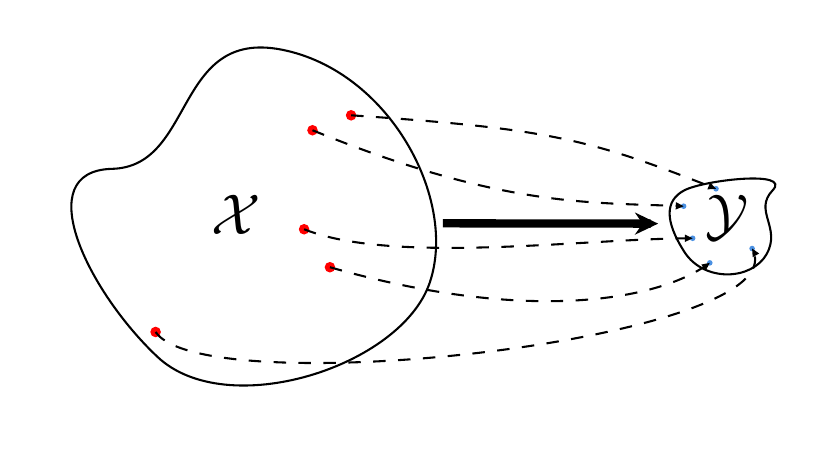
\begin{tikzpicture}[x=0.75pt,y=0.75pt,yscale=-0.6,xscale=0.6]
%uncomment if require: \path (0,300); %set diagram left start at 0, and has height of 300

%Shape: Regular Polygon [id:dp7047826808938766] 
\draw   (505.82,128.5) .. controls (521.58,120.27) and (592.49,112.04) .. (576.73,128.5) .. controls (560.97,144.97) and (583.82,158.14) .. (572,179.54) .. controls (560.18,200.94) and (521.58,202.58) .. (505.82,177.89) .. controls (490.06,153.2) and (490.06,136.74) .. (505.82,128.5) -- cycle ;
%Shape: Regular Polygon [id:dp28457392595956066] 
\draw   (182.32,15.52) .. controls (268.72,32.31) and (324.31,135.62) .. (301.3,202.88) .. controls (278.28,270.15) and (138.47,314.59) .. (82.84,262.29) .. controls (27.2,209.99) and (-20.63,112.91) .. (46.25,111.25) .. controls (113.13,109.59) and (95.91,-1.27) .. (182.32,15.52) -- cycle ;
%Straight Lines [id:da7059819659741645] 
\draw [line width=3]    (312,155) -- (478.75,155.24) ;
\draw [shift={(484.75,155.25)}, rotate = 180.08] [fill={rgb, 255:red, 0; green, 0; blue, 0 }  ][line width=0.08]  [draw opacity=0] (18.75,-9.01) -- (0,0) -- (18.75,9.01) -- (12.45,0) -- cycle    ;
%Shape: Circle [id:dp8333984030915326] 
\draw  [draw opacity=0][fill={rgb, 255:red, 255; green, 0; blue, 0 }  ,fill opacity=1 ] (196.25,159.75) .. controls (196.25,157.4) and (198.15,155.5) .. (200.5,155.5) .. controls (202.85,155.5) and (204.75,157.4) .. (204.75,159.75) .. controls (204.75,162.1) and (202.85,164) .. (200.5,164) .. controls (198.15,164) and (196.25,162.1) .. (196.25,159.75) -- cycle ;
%Shape: Circle [id:dp8350406714920023] 
\draw  [draw opacity=0][fill={rgb, 255:red, 255; green, 0; blue, 0 }  ,fill opacity=1 ] (234,68.25) .. controls (234,65.9) and (235.9,64) .. (238.25,64) .. controls (240.6,64) and (242.5,65.9) .. (242.5,68.25) .. controls (242.5,70.6) and (240.6,72.5) .. (238.25,72.5) .. controls (235.9,72.5) and (234,70.6) .. (234,68.25) -- cycle ;
%Shape: Circle [id:dp8078045840848124] 
\draw  [draw opacity=0][fill={rgb, 255:red, 255; green, 0; blue, 0 }  ,fill opacity=1 ] (203,80.25) .. controls (203,77.9) and (204.9,76) .. (207.25,76) .. controls (209.6,76) and (211.5,77.9) .. (211.5,80.25) .. controls (211.5,82.6) and (209.6,84.5) .. (207.25,84.5) .. controls (204.9,84.5) and (203,82.6) .. (203,80.25) -- cycle ;
%Shape: Circle [id:dp9196608519155977] 
\draw  [draw opacity=0][fill={rgb, 255:red, 255; green, 0; blue, 0 }  ,fill opacity=1 ] (217,190.25) .. controls (217,187.9) and (218.9,186) .. (221.25,186) .. controls (223.6,186) and (225.5,187.9) .. (225.5,190.25) .. controls (225.5,192.6) and (223.6,194.5) .. (221.25,194.5) .. controls (218.9,194.5) and (217,192.6) .. (217,190.25) -- cycle ;
%Shape: Circle [id:dp5247997255970858] 
\draw  [draw opacity=0][fill={rgb, 255:red, 255; green, 0; blue, 0 }  ,fill opacity=1 ] (77,242.25) .. controls (77,239.9) and (78.9,238) .. (81.25,238) .. controls (83.6,238) and (85.5,239.9) .. (85.5,242.25) .. controls (85.5,244.6) and (83.6,246.5) .. (81.25,246.5) .. controls (78.9,246.5) and (77,244.6) .. (77,242.25) -- cycle ;
%Shape: Circle [id:dp5977186799099233] 
\draw  [draw opacity=0][fill={rgb, 255:red, 74; green, 144; blue, 226 }  ,fill opacity=1 ] (529,127.25) .. controls (529,126.01) and (530.01,125) .. (531.25,125) .. controls (532.49,125) and (533.5,126.01) .. (533.5,127.25) .. controls (533.5,128.49) and (532.49,129.5) .. (531.25,129.5) .. controls (530.01,129.5) and (529,128.49) .. (529,127.25) -- cycle ;
%Shape: Circle [id:dp9077147150301588] 
\draw  [draw opacity=0][fill={rgb, 255:red, 74; green, 144; blue, 226 }  ,fill opacity=1 ] (510.25,167) .. controls (510.25,165.76) and (511.26,164.75) .. (512.5,164.75) .. controls (513.74,164.75) and (514.75,165.76) .. (514.75,167) .. controls (514.75,168.24) and (513.74,169.25) .. (512.5,169.25) .. controls (511.26,169.25) and (510.25,168.24) .. (510.25,167) -- cycle ;
%Shape: Circle [id:dp42007024913382485] 
\draw  [draw opacity=0][fill={rgb, 255:red, 74; green, 144; blue, 226 }  ,fill opacity=1 ] (558,175.25) .. controls (558,174.01) and (559.01,173) .. (560.25,173) .. controls (561.49,173) and (562.5,174.01) .. (562.5,175.25) .. controls (562.5,176.49) and (561.49,177.5) .. (560.25,177.5) .. controls (559.01,177.5) and (558,176.49) .. (558,175.25) -- cycle ;
%Shape: Circle [id:dp0830273454483047] 
\draw  [draw opacity=0][fill={rgb, 255:red, 74; green, 144; blue, 226 }  ,fill opacity=1 ] (524,186.75) .. controls (524,185.51) and (525.01,184.5) .. (526.25,184.5) .. controls (527.49,184.5) and (528.5,185.51) .. (528.5,186.75) .. controls (528.5,187.99) and (527.49,189) .. (526.25,189) .. controls (525.01,189) and (524,187.99) .. (524,186.75) -- cycle ;
%Shape: Circle [id:dp37881764730400724] 
\draw  [draw opacity=0][fill={rgb, 255:red, 74; green, 144; blue, 226 }  ,fill opacity=1 ] (503,141.25) .. controls (503,140.01) and (504.01,139) .. (505.25,139) .. controls (506.49,139) and (507.5,140.01) .. (507.5,141.25) .. controls (507.5,142.49) and (506.49,143.5) .. (505.25,143.5) .. controls (504.01,143.5) and (503,142.49) .. (503,141.25) -- cycle ;
%Curve Lines [id:da3052542411903666] 
\draw  [dash pattern={on 4.5pt off 4.5pt}]  (221.25,190.25) .. controls (378.85,235.31) and (483.09,217.31) .. (524.41,188.09) ;
\draw [shift={(526.25,186.75)}, rotate = 143.13] [fill={rgb, 255:red, 0; green, 0; blue, 0 }  ][line width=0.08]  [draw opacity=0] (6.25,-3) -- (0,0) -- (6.25,3) -- cycle    ;
%Curve Lines [id:da23141699655144976] 
\draw  [dash pattern={on 4.5pt off 4.5pt}]  (238.25,68.25) .. controls (397.95,79.2) and (428.69,86.92) .. (529.72,126.65) ;
\draw [shift={(531.25,127.25)}, rotate = 201.49] [fill={rgb, 255:red, 0; green, 0; blue, 0 }  ][line width=0.08]  [draw opacity=0] (6.25,-3) -- (0,0) -- (6.25,3) -- cycle    ;
%Curve Lines [id:da07636686680396754] 
\draw  [dash pattern={on 4.5pt off 4.5pt}]  (207.25,80.25) .. controls (359.22,142.13) and (428.61,138.09) .. (502.99,141.15) ;
\draw [shift={(505.25,141.25)}, rotate = 182.47] [fill={rgb, 255:red, 0; green, 0; blue, 0 }  ][line width=0.08]  [draw opacity=0] (6.25,-3) -- (0,0) -- (6.25,3) -- cycle    ;
%Curve Lines [id:da746662002529473] 
\draw  [dash pattern={on 4.5pt off 4.5pt}]  (81.25,242.25) .. controls (120.11,299.92) and (591.43,248.79) .. (561.32,177.42) ;
\draw [shift={(560.25,175.25)}, rotate = 60.66] [fill={rgb, 255:red, 0; green, 0; blue, 0 }  ][line width=0.08]  [draw opacity=0] (6.25,-3) -- (0,0) -- (6.25,3) -- cycle    ;
%Curve Lines [id:da05249635073342762] 
\draw  [dash pattern={on 4.5pt off 4.5pt}]  (200.5,159.75) .. controls (271.53,188.21) and (424.65,167.42) .. (509.94,167.01) ;
\draw [shift={(512.5,167)}, rotate = 180] [fill={rgb, 255:red, 0; green, 0; blue, 0 }  ][line width=0.08]  [draw opacity=0] (6.25,-3) -- (0,0) -- (6.25,3) -- cycle    ;

% Text Node
\draw (124,130) node [anchor=north west][inner sep=0.75pt]  [font=\huge]  {$\mathcal{{\displaystyle X}}$};
% Text Node
\draw (520,130) node [anchor=north west][inner sep=0.75pt]  [font=\huge]  {${\displaystyle \mathcal{Y}}$};
\end{tikzpicture}
\end{figure}
%%%%%%%%%%%%%%%%%%%%%%%%%%%%%%%%%%%%%%%%%%%%%%%%%%%%%%%%%%%%%%%%%%%%%%%%%%%
%%%%%%%%%%%%%%%%%%%%%%%%%%%%%%%%%%%%%%%%%%%%%%%%%%%%%%%%%%%%%%%%%%%%%%%%%%%

Unfortunately, there is an issue with the above approach: \emph{it is not possible}. That is, \emph{no matter what mapping we choose, there will be a set of $\ns$ elements mapped to fewer than $\ns$ points.} 
\begin{fact}[Pigeonhole Principle]
    Fix any two sets $\cX,\cY$ with $\green{m} > \green{m'}$. Then, for any mapping $h\colon \cX \to \cY$, there exists a set $S\subseteq \cX$ of $\flr{\frac{\green{m}-1}{\green{m'}}}+1 \geq 2$ elements all mapped to the same value in $\cY$.
\end{fact}
Importantly, this ``bad set of elements'' depends on the function $h$. This is merely telling us that, \emph{if} we do this mapping (``hashing'') from a large universe $\cX$ to a smaller set $\cY$ \emph{deterministically}, then there will be a \emph{worst-case} set of elements for which our strategy fails catastrophically. But what if we did things \emph{at random}?

\noindent We can consider three options:
\begin{itemize}
    \item \emph{The data is randomly distributed:} maybe our $\ns$ elements are not worst-case, but ``typical'' in some way, and we can model that as if they were chosen uniformly at random in $\cX$. Then the above argument does not go through, and we could use a single, deterministic hash function $h\colon \cX \to \cY$ while still getting good guarantees on average (over the randomness of the data). The main issue is that this is not a very realistic assumption, and what we can prove under this assumption will be more a heuristic as to why we could hope things to work in practice than a rigorous guarantee. Still, better than no guarantees at all.
    \item \emph{The hash function is totally random:} This would be nice. Then all the values $\{h(x)\}_{x\in \cX}$ are independent, uniformly distributed in $\cY$ we can bring in all the tools we have seen to analyze random variables in order to check the probability of a collision, the average number of elements hashed to a bucket $y\in \cY$, the maximum number of elements hashed to any bucket, etc. The main issue is that this will not solve our space issue: a totally random function takes a \emph{lot} of space to store, basically
    \[
        \green{m} \log_2 \green{m'} 
    \]
    bits: even worse than the array-based solution! We could try to only define $h$ on-the-fly, by generating $h(x)$ at random only the first time we need to hash $x\in\cX$. This would only require $\ns \log_2 \green{m'}$ bits of space\dots but now, we need to be consistent, and that means first checking if we already decided the value of $h(x)$ earlier. And for that, we need a dictionary~--~that's the problem we are trying to solve in the first place!
    \item \emph{The hash function is ``somewhat random'':} since a single hash function (deterministic) is bad (for collisions), and a truly uniform hash function (picking a function uniformly at random from all $(\green{m'})^{\green{m}}$ functions from $\cX$ to $\cY$) is also bad (for space), we could try to pick $h$ uniformly at random from a much smaller set of functions $\green{\mathcal{H}}$. Such an $h$ will only require $\log_2 |\green{\mathcal{H}}|$ bits to store, so if we can design $\green{\mathcal{H}}$ to be both small enough that this is space-efficient, and large enough that taking a random $h$ from it looks like we are picking a truly random function, then we are in good shape. And we are lucky: we have had a glimpse of these \emph{hash families} in Chapter~4, and \emph{they exist}.  % \cref{chap:derandomization}
\end{itemize}
Let us start with some more on these hash families: recall the notion of a \emph{strongly universal hash family} $\green{\mathcal{H}}$ from~\cref{def:universal:pairwise:hash}, which was asking that, for any \emph{pair} of distinct $x,x'\in \cX$, the two values $h(x),h(x')$ behave exactly (over the random choice of $h$ from $\green{\mathcal{H}}$) like two independent and uniformly distributed elements in $\cY$. We saw that such a family $\green{\mathcal{H}}$ of size only $2^{\clg{\log(\green{m}+1)}}$ existed for the case $|\cY|=2$ (\cref{fact:pairwise:hash:functions}).\marginnote{One can also ask for more than just pairwise independence, and require that, for any $k$-tuple of distinct $x_1,\dots, x_k\in \cX$, their hashed values $h(x_1),\dots, h(x_k)$ behave like $k$ independent uniformly random values in $\cY$. This is called a family of \emph{$k$-wise independent hash functions}, and again for the specific case of $|\cY|=2$ can be achieved with a family $\green{\mathcal{H}}$ of size $2^{O(\log \green{m})}$.}

\noindent For the general case, we can invoke the following result:\footnote{Try to prove it! This is similar to one of the exercises in Tutorial~4.}
\begin{theorem}
 Fix a prime number $p \geq 2$ and an integer $k \geq 1$. For given $a = (a_0,a_1,\dots,a_k)\in \Z_p^{k+1}$, define the function $h_a\colon \Z_p^k \to \Z_p$ by
\[
    h_a(x) = a_0 + \sum_{i=1}^k a_i x_i \bmod p, \qquad x \in \Z_p^k
\]
and let $\green{\mathcal{H}} = \{h_a\}_{a\in \Z_p^{k+1}}$. Then  $\green{\mathcal{H}}$ is a strongly universal hash family of size $|\green{\mathcal{H}}| = 2^{(k+1)\log_2 p}$.
\end{theorem}
In particular, by Bertrand's postulate, for every $\green{m'}$ there exists a prime number $\green{m'} \leq p < 2\green{m'}$. By choosing the smallest integer $k$ such that $p^k \geq \green{m}$, we get a strongly universal hash family from $\cX$ to some $\cY$ of cardinality $O(\green{m'})$, of size $2^{(k+1)\log_2 p} = 2^{O(k \log \green{m'})} = 2^{O(\log\green{m})}$. A little cumbersome, but it works.\smallskip

Still, strongly universal hash families are a very\dots strong (!) notion. For hash tables, all we need, in the end, is to have as few \emph{collisions} among hash values are possible: so it makes sense to only ask for this, which brings us to the (weaker) notion of \sout{strongly} \emph{universal hash family}:
\begin{definition}
    \label{def:universal:pairwise:hash}
    A family of functions $\green{\mathcal{H}} \subseteq \{h\colon \cX \to \cY\}$ is a \emph{universal hash family}, if, for every $x,x'\in \cX$ with $x\neq x'$,
    \[
        \probaDistrOf{h\sim \green{\mathcal{H}}}{ h(x) = h(x')  } \leq \frac{1}{|\mathcal{Y}|}
    \]
    where the probability is over the uniformly random choice of~$\green{h}\in\green{\mathcal{H}}$.
\end{definition}
Why this RHS? From Chapter~3 on Balls and Bins, we know that $\frac{1}{|\mathcal{Y}|}$ is the collision probability of two independent uniformly random values in $\mathcal{Y}$: so this definition is basically asking to do, collision-wise, at least as well as if each pair of hashed values behaved like two independent uniform random variables. And asking for an inequality instead of an equality just gives us more freedom when designing our $\green{\mathcal{H}}$, so why not?\marginnote{We will see in the tutorial that it is possible to build universal hash families for which the inequality is strict for \emph{some} pairs $x,x'$.}

This second notion will usually be enough for hash tables. But is it \emph{actually} weaker? As it turns out, yes:
\begin{lemma}
    Every strongly universal hash family is also a universal hash family. Moreover, there exist universal hash families which are not strongly universal.
\end{lemma}
\begin{proof}
    See Tutorial~4.
\end{proof}
To provide an example of a relatively simple (and small) universal hash family, fix any prime number $\green{m} \leq p < 2\green{m}$ and invoke the following construction:
\begin{theorem}
 Fix a prime number $p$. For given integers $a,b$, define the function $h_{a,b}\colon \Z_p\to [\green{m'}]$ by
\[
    h_a(x) = (ax + b \bmod p) \bmod \green{m'}, \qquad x \in \Z_p
\]
and let $\smash{\green{\mathcal{H}} = \{h_{a,b}\}_{\substack{1\leq a < p\\0\leq b <p}}}$. Then  $\green{\mathcal{H}}$ is a universal hash family of size $|\green{\mathcal{H}}| \leq 2^{2\log_2 p}$.
\end{theorem}
\begin{proof}
    The last part is clear, as $|\green{\mathcal{H}}| = p(p-1)$ (number of choices for the pair $(a,b)$.) To see that it is a universal hash family, note that if $x,x'\in\Z_p$ are distinct and $1\leq a<p$ , then $a$ and $x-x'$ are both among the $p-1$ invertible elements of $\Z_p$ (which is a field since $p$ is prime). This implies $ax+b \neq ax'+b \bmod p$. As a result, again in the field $\Z_p$, the linear system
    \begin{align*}
        ax + b &= y  \\
        ax' + b &= y'
    \end{align*}
    has a unique solution in $\Z_p\setminus\{0\}\times \Z_p$ for distinct $y,y'\in \Z_p$ (and no solution for $y=y'$): $a = (x-x')^{-1}(y-y')$ and $b = a(y'-y)^{-1}(yx'-y'x)$. The probability that the two independently chosen $a$ and $b$ take these two unique values is $\frac{1}{p-1}\cdot \frac{1}{p}$. We thus have, over the random choice of $1\leq a < p$, $0\leq b< p$, that
    \begin{align*}
        \probaDistrOf{a,b}{ax+b = y \bmod p, ax'+b = y'\bmod p} 
        = \begin{cases}
        0 &\text{if } y = y' \bmod p \\
        \frac{1}{p(p-1)} &\text{if } y \neq y' \bmod p
        \end{cases}
        \end{align*}
        Finally, $h_{a,b}(x)=h_{a,b}(x')$ if, and only if, $ax+b=y$ and $ax'+b=y'$ for two values $y,y' \in \Z_p$ such that $y=y' \bmod \green{m'}$. For any of the $p$ choices of $y\in \Z_p$, there are at most $\flr{p/\green{m'}}$ such choices of $y'\in \Z_p$: 
        \[
        y+\green{m'}, y+2\green{m'}, \dots, y+\flr{p/\green{m'}}\cdot \green{m'}
        \]
        and so
        \begin{align*}
        \probaDistrOf{a,b}{h_{a,b}(x)=h_{a,b}(x')}
        &\leq p\cdot \flr{\frac{p}{\green{m'}}}\cdot \frac{1}{p(p-1)} \\
        &\leq  p\cdot \frac{p-1}{\green{m'}}\cdot \frac{1}{p(p-1)}
        = \frac{1}{\green{m'}}
        \end{align*}
        where we used that, since $p$ is prime, $\flr{\frac{p}{\green{m'}}} = \flr{\frac{p-1}{\green{m'}}} \leq \frac{p-1}{\green{m'}}$.
\end{proof}
The above shows that, indeed, \emph{we have good universal hash families} (and even strongly universal ones if needed), with hash functions very easy to evaluate on any given input: so in what follows, we will, unless specified otherwise, go with the third option of ``somewhat random hash functions.'' The name of the game is to establish every statement we want to prove as if we were in the ``second option'' (the most convenient for us!), and at the end check the proof to verify we only used randomness in a way consistent with the third. This typically means relying on linearity of expectation and variance-based arguments such as Chebyshev's inequality, but no Chernoff or Hoeffding bounds (as the versions we have seen in this class require full independence).\marginnote{There exist Chernoff-type bounds using limited independence, but this is beyond the scope of these lecture notes.}

\paragraph{Alright, so what \emph{is} a hash table?} We finally get to it. A hash table consists of 3 things:
\begin{itemize}
    \item A hash function $h$ from the universe $\cX$ to a much smaller set $\cY$, usually of size $\green{m'}=|\cY|=O(\ns)$. \emph{[This $h$ is, at the initialization of the data structure, drawn from a ``good'' hash family $\green{\mathcal{H}}$]};
    \item An array $\orange{A}$ of size $\green{m'}$, where $\orange{A}[h(x)]$ will indicate whether element $x\in\cX$ is in the data structure; and
    \item a strategy to handle collisions in when two distinct $x,x'\in\cX$ end up in the same bucket (cell) of $\orange{A}$ because they have the same hash value (\ie $h(x)=h(x')$).
\end{itemize}
You may be wondering at this point~--~what is this third bullet? Did not we do all this hoping to \emph{minimize} the probability of collisions? Why do we still have to worry (and handle) them?

%%%%%%%%%%%%%%%%%%%%%%%%%%%%%%%%%%%%%%%%%%%%%%%%%%%%%%%%%%%%%%%%%%%%%%%%%%%
%%%%%%%%%%%%%%%%%%%%%%%%%%%%%%%%%%%%%%%%%%%%%%%%%%%%%%%%%%%%%%%%%%%%%%%%%%%
\begin{figure}
\tikzset{every picture/.style={line width=0.75pt}} %set default line width to 0.75pt     
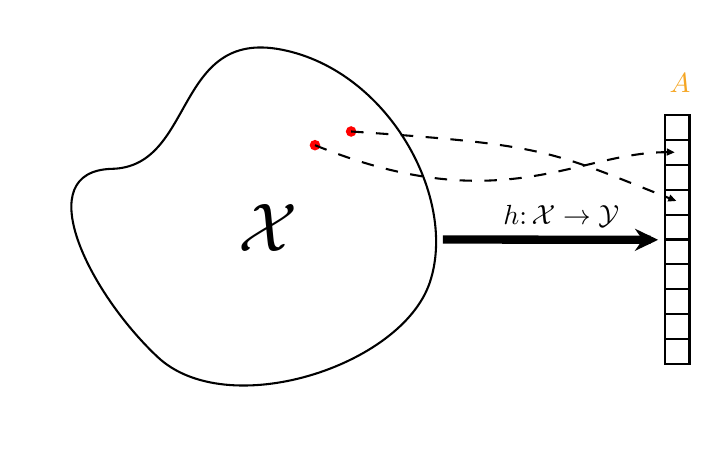
\begin{tikzpicture}[x=0.75pt,y=0.75pt,yscale=-0.6,xscale=0.6]
%uncomment if require: \path (0,300); %set diagram left start at 0, and has height of 300

%Shape: Regular Polygon [id:dp5892453846061058] 
\draw   (200.32,23.52) .. controls (286.72,40.31) and (342.31,143.62) .. (319.3,210.88) .. controls (296.28,278.15) and (156.47,322.59) .. (100.84,270.29) .. controls (45.2,217.99) and (-2.63,120.91) .. (64.25,119.25) .. controls (131.13,117.59) and (113.91,6.73) .. (200.32,23.52) -- cycle ;
%Straight Lines [id:da5940227274966229] 
\draw [line width=3]    (330,176) -- (496.75,176.24) ;
\draw [shift={(502.75,176.25)}, rotate = 180.08] [fill={rgb, 255:red, 0; green, 0; blue, 0 }  ][line width=0.08]  [draw opacity=0] (18.75,-9.01) -- (0,0) -- (18.75,9.01) -- (12.45,0) -- cycle    ;
%Shape: Grid [id:dp5884380060790032] 
\draw  [draw opacity=0] (508,76) -- (528,76) -- (528,276) -- (508,276) -- cycle ; \draw    ; \draw   (508,96) -- (528,96)(508,116) -- (528,116)(508,136) -- (528,136)(508,156) -- (528,156)(508,176) -- (528,176)(508,196) -- (528,196)(508,216) -- (528,216)(508,236) -- (528,236)(508,256) -- (528,256) ; \draw   (508,76) -- (528,76) -- (528,276) -- (508,276) -- cycle ;
%Shape: Circle [id:dp7080915007017408] 
\draw  [draw opacity=0][fill={rgb, 255:red, 255; green, 0; blue, 0 }  ,fill opacity=1 ] (252,89.25) .. controls (252,86.9) and (253.9,85) .. (256.25,85) .. controls (258.6,85) and (260.5,86.9) .. (260.5,89.25) .. controls (260.5,91.6) and (258.6,93.5) .. (256.25,93.5) .. controls (253.9,93.5) and (252,91.6) .. (252,89.25) -- cycle ;
%Curve Lines [id:da44474204475477297] 
\draw  [dash pattern={on 4.5pt off 4.5pt}]  (256.25,89.25) .. controls (415.95,100.2) and (415.01,104.7) .. (515.72,144.4) ;
\draw [shift={(517.25,145)}, rotate = 201.49] [fill={rgb, 255:red, 0; green, 0; blue, 0 }  ][line width=0.08]  [draw opacity=0] (6.25,-3) -- (0,0) -- (6.25,3) -- cycle    ;
%Shape: Circle [id:dp43426133236609155] 
\draw  [draw opacity=0][fill={rgb, 255:red, 255; green, 0; blue, 0 }  ,fill opacity=1 ] (223,100.25) .. controls (223,97.9) and (224.9,96) .. (227.25,96) .. controls (229.6,96) and (231.5,97.9) .. (231.5,100.25) .. controls (231.5,102.6) and (229.6,104.5) .. (227.25,104.5) .. controls (224.9,104.5) and (223,102.6) .. (223,100.25) -- cycle ;
%Curve Lines [id:da27933594579127596] 
\draw  [dash pattern={on 4.5pt off 4.5pt}]  (227.25,100.25) .. controls (379.22,162.13) and (439.54,103.94) .. (513.75,105.92) ;
\draw [shift={(516,106)}, rotate = 182.47] [fill={rgb, 255:red, 0; green, 0; blue, 0 }  ][line width=0.08]  [draw opacity=0] (6.25,-3) -- (0,0) -- (6.25,3) -- cycle    ;

% Text Node
\draw (163.5,145.4) node [anchor=north west][inner sep=0.75pt]  [font=\Huge]  {$\mathcal{X}$};
% Text Node
\draw (509.5,39.9) node [anchor=north west][inner sep=0.75pt]    {$\textcolor[rgb]{0.96,0.65,0.14}{\boldsymbol{A}}$};
% Text Node
\draw (376,145.9) node [anchor=north west][inner sep=0.75pt]    {$h\colon \mathcal{X}\rightarrow \mathcal{Y}$};



\end{tikzpicture}
\end{figure}
%%%%%%%%%%%%%%%%%%%%%%%%%%%%%%%%%%%%%%%%%%%%%%%%%%%%%%%%%%%%%%%%%%%%%%%%%%%
%%%%%%%%%%%%%%%%%%%%%%%%%%%%%%%%%%%%%%%%%%%%%%%%%%%%%%%%%%%%%%%%%%%%%%%%%%%



The sad truth is that collisions are inevitable, no matter how carefully we design our hash functions; and, even worse, we already saw why! This is the birthday paradox.
\begin{fact}
    Suppose $\orange{A}$ is of size $\green{m'} \leq c\cdot \ns^2$, for some absolute constant $c>0$. Then, even if the hash function $h\colon\cX\to [\green{m'}]$ was truly random, or even if the $\ns$ data points were truly independent uniformly random elements of $\cX$, there would still be a $99\%$ probability at least two elements of the data structure are hashed to the same bucket of $\orange{A}$.
\end{fact}
It is even worse than that: since we would like to take $\green{m'}=O(\ns)$, we also have this other result we saw earlier\dots\marginnote{At least, for this one, we have some idea of how we could try and resolve it: the power of two choices might help? Peeking ahead, this is the idea behind Cuckoo Hashing.}
\begin{fact}
    Suppose $\orange{A}$ is of size $\green{m'} \leq c\cdot \ns$, for some absolute constant $c>0$. Then, even if the hash function $h\colon\cX\to [\green{m'}]$ was truly random, or even if the $\ns$ data points were truly independent uniformly random elements of $\cX$, the expected maximum load among all buckets of $\orange{A}$ would be $\bigOmega{\frac{\log\ns}{\log\log\ns}}$. That is, we would expect at least one of the buckets to have at least this many hash collisions.
\end{fact}
%After all, in the array above, all but $\ns$ out of $\green{m}$ locations of the array are use
\subsection{Handling collisions}
Fortunately, there are many strategies to handle collisions, each with its advantages and drawbacks. We can divide them in two broad families: \emph{separate chaining}, and \emph{open addressing}.
\paragraph{(Separate) chaining}
Separate chaining is the most natural strategy: everybody hash value gets a list! If several of our $\ns$ data points are hashed to the same bucket in $\orange{A}$, add them to a linked list! That is, $\orange{A}[y]$ will link to a list of all the elements $x$ we want to store such that $h(x)=y$. To implement the 3 operations, we then just delegate to the list stored in the bucket:
    \begin{itemize}
        \item$\textsc{Insert}(x)$: call $\orange{A}[h(x)].\textsc{Insert}(x)$
        \item$\textsc{Lookup}(x)$: return $\orange{A}[h(x)].\textsc{Lookup}(x)$
        \item$\textsc{Remove}(x)$: call $\orange{A}[h(x)].\textsc{Remove}(x)$
    \end{itemize}
%%%%%%%%%%%%%%%%%%%%%%%%%%%%%%%%%%%%%%%%%%%%%%%%%%%%%%%%%%%%%%%%%%%%%%%%%%%
%%%%%%%%%%%%%%%%%%%%%%%%%%%%%%%%%%%%%%%%%%%%%%%%%%%%%%%%%%%%%%%%%%%%%%%%%%%
\begin{figure}
\tikzset{every picture/.style={line width=0.75pt}} %set default line width to 0.75pt     
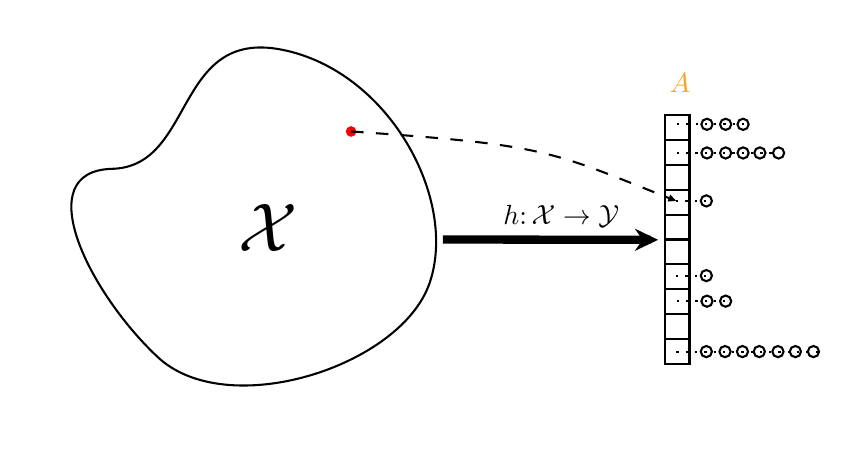
\begin{tikzpicture}[x=0.75pt,y=0.75pt,yscale=-0.6,xscale=0.6]
%uncomment if require: \path (0,300); %set diagram left start at 0, and has height of 300

%Shape: Regular Polygon [id:dp8090699692325243] 
\draw   (202.32,22.52) .. controls (288.72,39.31) and (344.31,142.62) .. (321.3,209.88) .. controls (298.28,277.15) and (158.47,321.59) .. (102.84,269.29) .. controls (47.2,216.99) and (-0.63,119.91) .. (66.25,118.25) .. controls (133.13,116.59) and (115.91,5.73) .. (202.32,22.52) -- cycle ;
%Straight Lines [id:da022629349356171446] 
\draw [line width=3]    (332,175) -- (498.75,175.24) ;
\draw [shift={(504.75,175.25)}, rotate = 180.08] [fill={rgb, 255:red, 0; green, 0; blue, 0 }  ][line width=0.08]  [draw opacity=0] (18.75,-9.01) -- (0,0) -- (18.75,9.01) -- (12.45,0) -- cycle    ;
%Shape: Grid [id:dp05145666164983498] 
\draw  [draw opacity=0] (510,75) -- (530,75) -- (530,275) -- (510,275) -- cycle ; \draw    ; \draw   (510,95) -- (530,95)(510,115) -- (530,115)(510,135) -- (530,135)(510,155) -- (530,155)(510,175) -- (530,175)(510,195) -- (530,195)(510,215) -- (530,215)(510,235) -- (530,235)(510,255) -- (530,255) ; \draw   (510,75) -- (530,75) -- (530,275) -- (510,275) -- cycle ;
%Shape: Circle [id:dp6479250592118756] 
\draw   (539.5,82.5) .. controls (539.5,80.01) and (541.51,78) .. (544,78) .. controls (546.49,78) and (548.5,80.01) .. (548.5,82.5) .. controls (548.5,84.99) and (546.49,87) .. (544,87) .. controls (541.51,87) and (539.5,84.99) .. (539.5,82.5) -- cycle ;
%Shape: Circle [id:dp34702826817417354] 
\draw   (554.5,82.5) .. controls (554.5,80.01) and (556.51,78) .. (559,78) .. controls (561.49,78) and (563.5,80.01) .. (563.5,82.5) .. controls (563.5,84.99) and (561.49,87) .. (559,87) .. controls (556.51,87) and (554.5,84.99) .. (554.5,82.5) -- cycle ;
%Shape: Circle [id:dp4536557388273843] 
\draw   (568.5,82.5) .. controls (568.5,80.01) and (570.51,78) .. (573,78) .. controls (575.49,78) and (577.5,80.01) .. (577.5,82.5) .. controls (577.5,84.99) and (575.49,87) .. (573,87) .. controls (570.51,87) and (568.5,84.99) .. (568.5,82.5) -- cycle ;
%Shape: Circle [id:dp8353479068292242] 
\draw   (539.5,105.5) .. controls (539.5,103.01) and (541.51,101) .. (544,101) .. controls (546.49,101) and (548.5,103.01) .. (548.5,105.5) .. controls (548.5,107.99) and (546.49,110) .. (544,110) .. controls (541.51,110) and (539.5,107.99) .. (539.5,105.5) -- cycle ;
%Shape: Circle [id:dp38555811039605437] 
\draw   (554.5,105.5) .. controls (554.5,103.01) and (556.51,101) .. (559,101) .. controls (561.49,101) and (563.5,103.01) .. (563.5,105.5) .. controls (563.5,107.99) and (561.49,110) .. (559,110) .. controls (556.51,110) and (554.5,107.99) .. (554.5,105.5) -- cycle ;
%Shape: Circle [id:dp7008873748312328] 
\draw   (568.5,105.5) .. controls (568.5,103.01) and (570.51,101) .. (573,101) .. controls (575.49,101) and (577.5,103.01) .. (577.5,105.5) .. controls (577.5,107.99) and (575.49,110) .. (573,110) .. controls (570.51,110) and (568.5,107.99) .. (568.5,105.5) -- cycle ;
%Shape: Circle [id:dp750804228542512] 
\draw   (582,105.5) .. controls (582,103.01) and (584.01,101) .. (586.5,101) .. controls (588.99,101) and (591,103.01) .. (591,105.5) .. controls (591,107.99) and (588.99,110) .. (586.5,110) .. controls (584.01,110) and (582,107.99) .. (582,105.5) -- cycle ;
%Shape: Circle [id:dp13100978706796573] 
\draw   (597,105.5) .. controls (597,103.01) and (599.01,101) .. (601.5,101) .. controls (603.99,101) and (606,103.01) .. (606,105.5) .. controls (606,107.99) and (603.99,110) .. (601.5,110) .. controls (599.01,110) and (597,107.99) .. (597,105.5) -- cycle ;
%Shape: Circle [id:dp9837665512770466] 
\draw   (539,144) .. controls (539,141.51) and (541.01,139.5) .. (543.5,139.5) .. controls (545.99,139.5) and (548,141.51) .. (548,144) .. controls (548,146.49) and (545.99,148.5) .. (543.5,148.5) .. controls (541.01,148.5) and (539,146.49) .. (539,144) -- cycle ;
%Shape: Circle [id:dp7642283303814478] 
\draw   (539,204) .. controls (539,201.51) and (541.01,199.5) .. (543.5,199.5) .. controls (545.99,199.5) and (548,201.51) .. (548,204) .. controls (548,206.49) and (545.99,208.5) .. (543.5,208.5) .. controls (541.01,208.5) and (539,206.49) .. (539,204) -- cycle ;
%Shape: Circle [id:dp6692954665359216] 
\draw   (539.5,224.5) .. controls (539.5,222.01) and (541.51,220) .. (544,220) .. controls (546.49,220) and (548.5,222.01) .. (548.5,224.5) .. controls (548.5,226.99) and (546.49,229) .. (544,229) .. controls (541.51,229) and (539.5,226.99) .. (539.5,224.5) -- cycle ;
%Shape: Circle [id:dp8910308062853909] 
\draw   (554.5,224.5) .. controls (554.5,222.01) and (556.51,220) .. (559,220) .. controls (561.49,220) and (563.5,222.01) .. (563.5,224.5) .. controls (563.5,226.99) and (561.49,229) .. (559,229) .. controls (556.51,229) and (554.5,226.99) .. (554.5,224.5) -- cycle ;
%Shape: Circle [id:dp21020217647833994] 
\draw   (539,265) .. controls (539,262.51) and (541.01,260.5) .. (543.5,260.5) .. controls (545.99,260.5) and (548,262.51) .. (548,265) .. controls (548,267.49) and (545.99,269.5) .. (543.5,269.5) .. controls (541.01,269.5) and (539,267.49) .. (539,265) -- cycle ;
%Shape: Circle [id:dp5092131007727523] 
\draw   (554,265) .. controls (554,262.51) and (556.01,260.5) .. (558.5,260.5) .. controls (560.99,260.5) and (563,262.51) .. (563,265) .. controls (563,267.49) and (560.99,269.5) .. (558.5,269.5) .. controls (556.01,269.5) and (554,267.49) .. (554,265) -- cycle ;
%Shape: Circle [id:dp6005647648405279] 
\draw   (568,265) .. controls (568,262.51) and (570.01,260.5) .. (572.5,260.5) .. controls (574.99,260.5) and (577,262.51) .. (577,265) .. controls (577,267.49) and (574.99,269.5) .. (572.5,269.5) .. controls (570.01,269.5) and (568,267.49) .. (568,265) -- cycle ;
%Shape: Circle [id:dp6056236374130685] 
\draw   (581.5,265) .. controls (581.5,262.51) and (583.51,260.5) .. (586,260.5) .. controls (588.49,260.5) and (590.5,262.51) .. (590.5,265) .. controls (590.5,267.49) and (588.49,269.5) .. (586,269.5) .. controls (583.51,269.5) and (581.5,267.49) .. (581.5,265) -- cycle ;
%Shape: Circle [id:dp6814289868642057] 
\draw   (596.5,265) .. controls (596.5,262.51) and (598.51,260.5) .. (601,260.5) .. controls (603.49,260.5) and (605.5,262.51) .. (605.5,265) .. controls (605.5,267.49) and (603.49,269.5) .. (601,269.5) .. controls (598.51,269.5) and (596.5,267.49) .. (596.5,265) -- cycle ;
%Shape: Circle [id:dp4003339160068812] 
\draw   (610.5,265) .. controls (610.5,262.51) and (612.51,260.5) .. (615,260.5) .. controls (617.49,260.5) and (619.5,262.51) .. (619.5,265) .. controls (619.5,267.49) and (617.49,269.5) .. (615,269.5) .. controls (612.51,269.5) and (610.5,267.49) .. (610.5,265) -- cycle ;
%Shape: Circle [id:dp5195042865870344] 
\draw   (625,265) .. controls (625,262.51) and (627.01,260.5) .. (629.5,260.5) .. controls (631.99,260.5) and (634,262.51) .. (634,265) .. controls (634,267.49) and (631.99,269.5) .. (629.5,269.5) .. controls (627.01,269.5) and (625,267.49) .. (625,265) -- cycle ;
%Straight Lines [id:da10849130917681804] 
\draw  [dash pattern={on 0.84pt off 2.51pt}]  (520,82.5) -- (577.5,82.5) ;
%Straight Lines [id:da8301322053157919] 
\draw  [dash pattern={on 0.84pt off 2.51pt}]  (519.75,105.5) -- (601.5,105.5) ;
%Straight Lines [id:da6070616319798346] 
\draw  [dash pattern={on 0.84pt off 2.51pt}]  (519.25,144) -- (543.5,144) ;
%Straight Lines [id:da9016627948586332] 
\draw  [dash pattern={on 0.84pt off 2.51pt}]  (519.75,224.5) -- (563.5,224.5) ;
%Straight Lines [id:da5771080093661222] 
\draw  [dash pattern={on 0.84pt off 2.51pt}]  (519.5,265) -- (634,265) ;
%Straight Lines [id:da7159109321410426] 
\draw  [dash pattern={on 0.84pt off 2.51pt}]  (519.25,204) -- (543.5,204) ;
%Shape: Circle [id:dp8642716773725309] 
\draw  [draw opacity=0][fill={rgb, 255:red, 255; green, 0; blue, 0 }  ,fill opacity=1 ] (254,88.25) .. controls (254,85.9) and (255.9,84) .. (258.25,84) .. controls (260.6,84) and (262.5,85.9) .. (262.5,88.25) .. controls (262.5,90.6) and (260.6,92.5) .. (258.25,92.5) .. controls (255.9,92.5) and (254,90.6) .. (254,88.25) -- cycle ;
%Curve Lines [id:da3950336012128167] 
\draw  [dash pattern={on 4.5pt off 4.5pt}]  (258.25,88.25) .. controls (417.95,99.2) and (417.01,103.7) .. (517.72,143.4) ;
\draw [shift={(519.25,144)}, rotate = 201.49] [fill={rgb, 255:red, 0; green, 0; blue, 0 }  ][line width=0.08]  [draw opacity=0] (6.25,-3) -- (0,0) -- (6.25,3) -- cycle    ;

% Text Node
\draw (165.5,144.4) node [anchor=north west][inner sep=0.75pt]  [font=\Huge]  {$\mathcal{X}$};
% Text Node
\draw (511.5,38.9) node [anchor=north west][inner sep=0.75pt]    {$\textcolor[rgb]{0.96,0.65,0.14}{\boldsymbol{A}}$};
% Text Node
\draw (378,144.9) node [anchor=north west][inner sep=0.75pt]    {$h\colon \mathcal{X}\rightarrow \mathcal{Y}$};
\end{tikzpicture}
\end{figure}
%%%%%%%%%%%%%%%%%%%%%%%%%%%%%%%%%%%%%%%%%%%%%%%%%%%%%%%%%%%%%%%%%%%%%%%%%%%
%%%%%%%%%%%%%%%%%%%%%%%%%%%%%%%%%%%%%%%%%%%%%%%%%%%%%%%%%%%%%%%%%%%%%%%%%%%
In that sense, it combines the hash table (which is based on the naive array-based approach) with the linked-list approach, in an attempt to get the best of both worlds. 
Let
\begin{equation}
    \label{def:load:hashtable}
\alpha = \frac{\ns}{\green{m'}}
\end{equation}
denote the \emph{load factor} of the hash table. For $\green{m'} = O(\ns)$, this will be a (small) constant. Then:\marginnote{Note that chaining allows the load $\alpha$ to be greater than $1$. The next strategy, open addressing, does not.}
\begin{itemize}
    \item the total space used will be 
    \[
    O(\log\green{m} + \green{m'} + \ns \log \green{m}) = O((1+\alpha)\green{m'} \log \green{m})
    \]
    (the cost of storing the hash function, and the total space used by the array itself and by all the lists: that last one is proportional to the numbers $\ns$ of elements currently stored).
    \item by linearity of expectation, the \emph{expected} time complexity of all 3 operations is $O(1+\alpha)$, since $\alpha$ is the expected size of any given list.
    \item \dots but (think of the max load argument), most likely than not we will have some of the buckets for which the list has size $\Omega(\log\ns/\log\log\ns)$.\marginnote{This leads, for those, to a performance comparable to that of the BST approach!} 
\end{itemize}

\marginnote{\TODO{} {Give more detail here? Empirical evaluation of the maximum load for the family of hash functions given above.}}
\paragraph{Open addressing}
Another approach to handle collisions is \emph{open addressing}, which itself comes in several variants. The basic idea is quite simple: instead of a single hash function, we have a sequence of hash functions $h_1,\dots,h_t,\dots, h_{\green{m'}}$. If we are trying to insert an element $x$ in the hash table, we look at the bucket $h_1(x)$: if it's already taken (collision!), then we go to $h_1(x)$: if taken, we look at $h_3(x)$; etc. We stop when we found an empty bucket.\footnote{If there is no empty bucket, then this means the hash table is full (the load factor is $\alpha=1$) and we need to increase $\green{m'}$ to resize $\orange{A}$~--~an expensive operation, as this means re-hashing all elements.}

That is, we have the following:
    \begin{itemize}
        \item$\textsc{Insert}(x)$: 
            \begin{algorithmic}
                \ForAll{$1\leq t\leq \green{m'}$}
                    \If{$\orange{A}[h_t(x)]=x$}
                        \State \Return \Comment{Already there}
                    \ElsIf{$\orange{A}[h_t(x)]=\emptyset$ or $\orange{A}[h_t(x)]=\bot$}
                        \State $\orange{A}[h_t(x)]\gets x$ \Comment{Insert it in the first available bucket}
                        \State \Return 
                    \EndIf
                \EndFor
            \end{algorithmic}
        \item$\textsc{Lookup}(x)$: 
            \begin{algorithmic}
                \ForAll{$1\leq t\leq \green{m'}$}
                    \If{$\orange{A}[h_t(x)]=x$}
                        \State \Return \yes
                    \ElsIf{$\orange{A}[h_t(x)]=\emptyset$}
                        \State \Return \no \Comment{If $x$ was present, it'd have been found earlier}
                    \EndIf
                \EndFor
            \end{algorithmic}
        \item$\textsc{Remove}(x)$: 
                    \begin{algorithmic}
                \ForAll{$1\leq t\leq \green{m'}$}
                    \If{$\orange{A}[h_t(x)]=x$}
                        \State $\orange{A}[h_t(x)]\gets \bot$ \Comment{Special symbol to indicate there was something before}
                        \State \Return
                    \ElsIf{$\orange{A}[h_t(x)]=\emptyset$}
                        \State \Return \Comment{If $x$ was present, it'd have been found earlier}
                    \EndIf
                \EndFor
            \end{algorithmic}
    \end{itemize}
You may wonder why we have this strange symbol $\bot$ when we remove an element $x$. The reason is that if we just emptied that bucket by (making it $\emptyset$), this would potentially mess up future lookups: we would not know when to stop searching! \medskip

But \emph{how do we choose this sequence of hash functions?} We would like a few things: first, to make sure we cover all possible buckets: namely, for every $x\in\cX$, we want
\[
(h_1(x),\dots, h_{\green{m'}}(x))
\]
to me a permutation of $\{0,1,2,\dots,\green{m'}\}$. This is to make sure we do explore all possible buckets when trying to lookup or insert an element, if we keep finding collisions. Second, we would like to be able to \emph{store} (and evaluate) them all succinctly. We had only one hash function before, and we went to great lengths to make sure it did not take too much space to store, only $O(\log \green{m})$ bits: now, if we have $\green{m'}$, we'd like to avoid blowing up our space usage by that factor! For $\green{m'}=O(\ns)$, that would use space $O(\ns \log \green{m})$\dots

Before discussing (briefly) some common choices for this sequence of hash functions, let us first analyze the resulting (expected) time complexities of our 3 methods, under some very idealized (and unrealistic) assumptions:
\begin{theorem}
    \label{theo:wsishful:addressing}
    Assume that our sequence of hash functions is such that, for every element $x\in\cX$, the (random) sequence $(h_1(x),\dots, h_{\green{m'}}(x))$ is a uniformly random permutation of $[\green{m'}]$. Then, for every $x\in\cX$, \textsc{Lookup} runs in expected time 
    \[
    \bigO{\frac{1}{1-\alpha}}
    \]
   where $\alpha$ is the \emph{load factor} of the hash table, as defined in~\eqref{def:load:hashtable}.
\end{theorem}
\begin{proof}
    Fix any $x\in\cX$. Since we want to upper bound the expected running time, it is enough to consider the case where $x$ is \emph{not} in the data structure (unsuccessful lookup), since otherwise the search will end earlier (once it finds $x$). So the time here will be the number of steps until an empty bucket is found (in which case $\textsc{Lookup}$ finally will return $\no$).
    
    By symmetry, the probability that any given bucket is empty is equal to $1-\frac{\ns}{\green{m'}}$. Let $T(\ns, \green{m'})$ be the time taken by an (unsuccessful) search for item $x$ in the hash table of size $\green{m'}$ containing $\ns$ hash values. If the first index checked corresponds to an empty bucket (with by the above happens with probability $\frac{\ns}{\green{m'}}$), then the search ends after this one step; otherwise, we continue on the remaining subarray of $\green{m'}-1$ buckets, containing the remaining $\ns-1$ hash values. And, crucially, the remaining sequence of hash functions values $(h_2(x),\dots, h_{\green{m'}}(x))$ is \emph{still} a uniformly random permutation of these remaining $\green{m'}-1$ buckets (all except the bucket $h_1(x)$, which has been looked at already). 
    So we have the recurrence relation:
    \[
        \bEE{T(\ns, \green{m'})} = 1 + \frac{\ns}{\green{m'}}\cdot  \bEE{T(\ns-1, \green{m'}-1)}
    \]
    We can then prove by induction (over $\ns$) that the solution is 
    \[
    \bEE{T(\ns, \green{m'})} \leq \frac{1}{1-\frac{\ns}{\green{m'}}}\,,
    \]
    which concludes the proof.
\end{proof}
With this in hand, here are some of the common strategies to implement open addressing:
\begin{itemize}
    \item Linear probing: forget about using completely distinct hash functions! We have \emph{one} hash function $h$, let us make the most out of it and just look at the next bucket at each step:
    \[
        h_t(x) = h(x)+(t-1) \bmod \green{m'}
    \]
    On the plus side, this is very good in terms of space complexity (we still only store \emph{one} hash function), and very fast to evaluate (as long as $h$ itself is fast to evaluate). How well does this do? The time complexity of any of the 3 functions is again related to the {load factor} of the hash table, and quickly degrades as $\alpha$ gets close to $1$. Namely, we have:
    \begin{theorem}[Knuth'62]
        Assume for simplicity that the hash function $h\colon \cX\to\cY$ is a truly random function, and furthermore that the loads of each bucket , $(|h^{-1}(y)|)_{y\in[\green{m'}}$, are independent. Then, the expected time complexities of \textsc{Insert}, \textsc{Lookup}, and \textsc{Remove} are all $\bigO{\frac{1}{(1-\alpha)^2}}$.
    \end{theorem}
    We will not prove this here, but this is actually quite surprising (and bad), and shows that linear probing actually performs much worse than one would think! Indeed, compare this to the wishful analysis of~\cref{theo:wsishful:addressing}.
    \item Quadratic probing: the same idea, but now
    \[
        h_t(x) = h(x)+c_1 t + c_2 t^2 \bmod \green{m'}
    \]
    for two constants $c_1,c_2$ with $c_2 \neq 0$ chosen somewhat arbitrarily (but in order to get a permutation of $\{0,1,2,\dots,\green{m'}\}$). This is supposed to incur less ``clustering'' of values than linear probing, while having the same advantages.
    \item Double hashing: we use \emph{two} hash functions, $h,g$, and set
        \[
        h_t(x) = h(x)+(t-1)\cdot g(x) \bmod \green{m'}
        \]
    \item Cuckoo hashing: this one is really neat, as it goes beyond \emph{expected} running times, and actually provides \emph{worst-case} running time guarantees for 2 out of 3 operations. This hashing strategy was proposed and analyzed by Pagh and Flemming in 2001,\cite{PaghR01,PaghR04} and relies on a beautiful idea you have seen in an earlier lecture: the power of two choices. Specifically, the data structure uses two hash tables, $h_1, \orange{A_1}$ and  $h_2, \orange{A_2}$. An element $x\in \cX$ can only be hashed to one of its two locations, either $\orange{A_1}[h_1(x)]$ or $\orange{A_2}[h_2(x)]$: so for lookups and removals, it suffices to check both of these.

        \begin{itemize}
        \item$\textsc{Lookup}(x)$: 
            \begin{algorithmic}
                \If{$\orange{A_1}[h_1(x)]=x$ or $\orange{A_2}[h_2(x)]=x$}
                        \State \Return \yes
                    \Else
                        \State \Return \no
                    \EndIf
            \end{algorithmic}
        \item$\textsc{Remove}(x)$: 
                    \begin{algorithmic}
                \If{$\orange{A_1}[h_1(x)]=x$}
                        \State $\orange{A_1}[h_1(x)] \gets \emptyset$
                \ElsIf{$\orange{A_2}[h_2(x)]=x$}
                        \State $\orange{A_2}[h_2(x)] \gets \emptyset$
                \EndIf
            \end{algorithmic}
    \end{itemize}

    For insertions, it is a bit more complicated. When inserting an element $x$, if either $\orange{A_1}[h_1(x)]$ or $\orange{A_2}[h_2(x)]$ is empty, we are done: we can insert $x$ to that empty slot. If both are currently occupied, say by two other elements $x'$ and $x''$\dots then, an \emph{eviction} occurs (which is where the ``cuckoo'' part of the name comes from. Cuckoos are\dots not very nice birds.). That is, $x$ takes the spot of $x'$, forcing $x'$ to go to its own other location in $\orange{A_2}$. If that location is empty, then $x'$ goes there and everyone is happy: but if \emph{another} element was there\dots then $x'$ takes that spot, forcing that element itself to go to its alternate location in the other hash table. And so on and so forth, until the cycle ends or the maximum number of evictions has been reached.
    \begin{itemize}
        \item$\textsc{Insert}(x)$: 
                    \begin{algorithmic}
                \If{$\orange{A_1}[h_1(x)]=\emptyset$}
                        \State $\orange{A_1}[h_1(x)] \gets x$
                \ElsIf{$\orange{A_2}[h_2(x)]=\emptyset$}
                        \State $\orange{A_2}[h_2(x)] \gets x$
                \Else
                    \State $T \gets 0$ \Comment{The evictions start}
                    \State $x' \gets \orange{A_1}[h_1(x)]$
                    \State $\orange{A_1}[h_1(x)] \gets x$
                    \While{$T < T_{\max}$}
                    \State $x'$ goes to $\orange{A_2}[h_2(x')]$, and if there was something there, that element now needs to move, etc.
                    \State $T\gets T+1$
                    \EndWhile                    
                \EndIf
            \end{algorithmic}
    \end{itemize}
    \begin{theorem}
        Cuckoo hashing achieves worst-case time $O(1)$ for \textsc{Lookup} and
\textsc{Remove}, and expected time $O(1)$ for \textsc{Insert}.
    \end{theorem}
    The guarantees for \textsc{Lookup} and \textsc{Remove} are immediate; the expected guarantee for \textsc{Insert}, however, is quite involved. We will not prove it here (but will discuss some of it during the tutorial).
\end{itemize}

\begin{remark}[And there is more!]
There are other strategies, such as 2-level hashing (where we use a second hash table for each bucket). We will see more during the tutorial.
\end{remark}
%\subsection{Applications}
%2-sum?
% Talk about "why do things appear to work so well" -- the Mitzenmacher--Vadhan paper? http://timroughgarden.org/f14/l/l16_old.pdf
%%%%%%%%%%%%%%%%%%%%%%%%%%%%%%%%%%%%%%%%
\subsection{Bloom filters}

As we saw above, a hash table allows us to store and retrieve data very quickly (in expectation, or ``for typical data''); the data structures never ``make mistakes'', since the result is always correct, and the only random aspect is the time complexity. But while they are typically faster and very space efficient, hash tables do still use some \emph{space}: if each element $x\in \cX$ takes $\log_2 \green{m}$ (where $\green{m} = |\cX|$) bits to store, a hash table will take $O(\ns\log \green{m})$ space to store $\ns$ elements. Which is very little, and usually alright, but \emph{sometimes} is not.
	
	In this short section, we will see a related data structure, the \emph{Bloom filter}, which uses much less space while still providing efficient access and insertion: only $O(\ns)$ space to store $\ns$ elements (regardless of how many bits an element takes to encode)! But this comes at a price: sometimes, the result of a query to the data structure will be wrong. However, when designed well, the frequency with which those mistakes occur is relatively low, and can be controlled.
	
	Let us start with what a Bloom filter is. For simplicity, here we will only allow insertions ($\textsc{Insert}$) and lookups ($\textsc{Lookup}$), but no deletions.\footnote{They could be implemented, but this adds quite a bit of complexity to the data structure.} The Bloom filter is an array $\orange{A}$ of size $\green{m'}$ (containing $\green{m'}$ bits, initialized to $0$), along with $\blue{k}$ distinct hash functions $h_1,\dots,h_{\blue{k}}$, each mapping the data universe $\cX$ to $[\green{m'}] = \{1,2,\dots,\green{m'}\}$:
	\[
		h_i\colon \cX \to \cY = [\green{m'}], \qquad i\in\{1,2,\dots,m\}
	\]
	where $\green{m'}$ and $\blue{k}$ are parameters to choose. Here is how it works: given an element $x\in \cX$,
	\begin{itemize}
	\item $\textsc{insert}(x)$ evaluates the $\blue{k}$ hash functions on $x$ and sets the bit of all $\blue{k}$ corresponding cells to $1$.
		\begin{algorithmic}
		  \Function{Insert}{$x$}
		  \ForAll{$1\leq i \leq \blue{k}$}
			  \State $\orange{A}[h_i(x)] \gets 1$
		  \EndFor
		  \EndFunction
		\end{algorithmic}
	\item $\textsc{Lookup}(x)$ evaluates the $\blue{k}$ hash functions on $x$ and checks that all the $\blue{k}$ bits in the corresponding cells are equal to $1$.
		\begin{algorithmic}
		  \Function{Lookup}{$x$}
		  \ForAll{$1\leq i \leq \blue{k}$}
			  \If{ $\orange{A}[h_i(x)] = 0$ }
			  	\State \Return \no
			  \EndIf
		  \EndFor
		  \State \Return \yes
		  \EndFunction
		\end{algorithmic}
	\end{itemize}'

 That's all! In the rest of this lecture, we will try to see what this does, how to analyze the performance, and see how to choose the parameter $\blue{k}$ (number of hash functions).

 \paragraph{What type of ``mistakes'' can $\textsc{Lookup}$ make?}

 A Bloom filter can only make one type of errors:  \emph{false positives} (returning \yes when the element is not in the data structure), never any \emph{false negative} (returning \no although the element \emph{is} in the data structure). This is because once its corresponding bits are set to $1$, the element will always be reported as present. But a non-present element might have its $\blue{k}$ bits set to $1$ by several other elements. Here's an example with $m=3$, $N=10$, and $\cX=\{1,2,3,4\}$: consider the hash functions
\begin{center}
\begin{tabular}{|c|c|c|c|}\hline
	& $h_1$ & $h_2$& $h_3$ \\\hline
	1&1&5&10\\\hline
	2&9&4&6\\\hline
	3&1&6&3 \\\hline
	4&7&3&8\\\hline
\end{tabular}
\end{center}
~\newline

Say we insert $S=\{1,2,4\}$: the corresponding bits set to $1$ will be (indexing starting at $1$)
\begin{align*}
	1 &\leadsto \orange{A}[1], \orange{A}[5], \orange{A}[10] \\
	2 &\leadsto \orange{A}[9], \orange{A}[4], \orange{A}[6] \\
	4 &\leadsto \orange{A}[7], \orange{A}[3], \orange{A}[8]
\end{align*}

Now, when calling $\textsc{Lookup}(3)$, we will check if the bits $\orange{A}[1], \orange{A}[6], \orange{A}[3]$ are all equal to $1$. And they all are, so $\textsc{Lookup}(3)$ will return \yes even though $3$ was \emph{not} inserted.

\paragraph{Space complexity}
Assuming each hash function can be stored in $O(\log\green{m})$ space and takes $O(1)$ time to evaluate, the space complexity of the Bloom filter is
\begin{equation}
    \label{eq:bloomfiler:space}
    O(\blue{k}\log\green{m} + \green{m'})
\end{equation}
and the (worst-case) time complexities of $\textsc{Insert}$ and $\textsc{Lookup}$ are $O(\blue{k})$.

\paragraph{Error probability}
Under the idealized (that is: wrong) simplifying assumption that all $\blue{k}$ hash functions behave like independent, truly random functions, one can show that the probability that $\textsc{Lookup}$ makes an error after $\ns$ elements have been inserted in the data structure is
\begin{equation}
\label{eq:bloomfiler:error}
\Paren{1-\Paren{1-\frac{1}{\green{m'}}^{\ns \blue{k}}}}^{\blue{k}} \approx 
\Paren{1-e^{-\frac{\ns \blue{k}}{\green{m'}}}}^{\blue{k}}
\end{equation}
By looking at the tradeoff between space \eqref{eq:bloomfiler:space} and error probability \eqref{eq:bloomfiler:error}, one can then set the parameters $\blue{k}$ and $\green{m'}$ as desired. For instance, for a fixed $\ns$ and a target value of space $\green{m'}$, we can derive the optimal value of $\blue{k}$ to set in order to minimize the probability of error.